\documentclass[11pt,UTF8,fontset=fandol]{ctexart}
\usepackage{amsmath,amssymb,amsfonts}
\usepackage{graphicx,float,caption,subcaption}
\usepackage{booktabs,array,multirow,makecell}
\usepackage{geometry,enumitem,xcolor}
\usepackage[hidelinks]{hyperref}
\usepackage{url}
\usepackage{pdfpages}
\geometry{margin=2.3cm}
\graphicspath{{/Users/yye/project/论文/assets/got/}}
\captionsetup{font=small,labelfont=bf}
\setlength{\parskip}{0.4em}

% 用于原样展示英文示例 prompt 的环境（附录数据，不翻译）
\usepackage{listings}
\lstset{
  basicstyle=\ttfamily\scriptsize,
  breaklines=true,
  breakatwhitespace=false,
  columns=fullflexible,
  frame=single,
  framesep=4pt,
  xleftmargin=4pt,
  xrightmargin=4pt,
  aboveskip=4pt,
  belowskip=4pt,
  keepspaces=true,
  showstringspaces=false,
  literate={”}{{"}}1 {“}{{"}}1 {’}{{'}}1 {–}{{-}}1 {…}{{...}}1
}
\newcommand{\promptbox}[1]{\par\noindent\begin{lstlisting}#1\end{lstlisting}}

\title{\textbf{思维之图：用大语言模型解决复杂问题}}

\author{Maciej Besta\textsuperscript{1*}, Nils Blach\textsuperscript{1*}, Ales Kubicek\textsuperscript{1}, Robert Gerstenberger\textsuperscript{1},\\
Michał Podstawski\textsuperscript{2}, Lukas Gianinazzi\textsuperscript{1}, Joanna Gajda\textsuperscript{3}, Tomasz Lehmann\textsuperscript{3},\\
Hubert Niewiadomski\textsuperscript{3}, Piotr Nyczyk\textsuperscript{3}, Torsten Hoefler\textsuperscript{1}\\[0.4em]
\textsuperscript{1}ETH Zurich（苏黎世联邦理工学院），\textsuperscript{2}Warsaw University of Technology（华沙理工大学），\textsuperscript{3}Cledar\\
\texttt{bestam@inf.ethz.ch, nils.blach@inf.ethz.ch, htor@inf.ethz.ch}\\[0.3em]
\small（\textsuperscript{*}为同等贡献作者）}

\date{}

\begin{document}
\maketitle

\begin{abstract}
我们提出思维之图（Graph of Thoughts, GoT）：一个能够提升大语言模型（large language models, LLMs）提示（prompting）能力的框架，其能力超越了链式思维（Chain-of-Thought）或思维之树（Tree of Thoughts, ToT）等范式所提供的水平。GoT 的核心思想与首要优势在于，能够把大语言模型生成的信息建模为任意图（arbitrary graph），其中信息单元（即“LLM 思维”，LLM thoughts）是顶点，而边对应于这些顶点之间的依赖关系。这一方法使得我们能够将任意的 LLM 思维组合成协同增效的结果，提炼出整个思维网络的精华，或借助反馈回路（feedback loop）来强化思维。我们说明 GoT 在不同任务上相对于现有最佳方法（state of the art）具有优势，例如在排序任务上，其质量比 ToT 提升了 62\%，同时成本降低了 31\% 以上。我们确保 GoT 可以用新的思维变换（thought transformation）进行扩展，因而可以用来引领新的提示方案。本工作使大语言模型推理更加贴近人类思维或大脑机制（例如递归），二者都构成了复杂的网络。

\vspace{0.5em}
\noindent 网站与代码：\url{https://github.com/spcl/graph-of-thoughts}
\end{abstract}

\section{引言}

大语言模型（LLMs）正在席卷整个人工智能（AI）领域。近年来，主要基于仅解码器（decoder-only）Transformer 变体 [65] 的模型迅速发展，例如 GPT [13, 14, 53, 54]、PaLM [19] 或 LLaMA [63]。

提示工程（prompt engineering）是一种资源高效的方法，可用于解决各类 LLM 任务。简而言之，人们在发送给 LLM 的输入中包含任务描述。如果这一描述表述得当，LLM 就会利用其基于词元（token）的自回归（autoregressive）文本生成机制来求解任务。这类提示可以包含带有解答的示例任务（少样本提示，few-shot prompting，也称为上下文学习，in-context learning, ICL），甚至可以完全不含示例任务（零样本提示，zero-shot prompting）。近年来研究表明，这一机制可以用于求解涉及数学、常识或符号推理（symbolic reasoning）的一大类任务。

链式思维（Chain-of-Thought, CoT）[71] 是一种提示方法，除任务输入/输出之外，还在提示中包含推理的中间步骤（中间“思维”，intermediate “thoughts”）。研究表明，CoT 能够在不进行任何模型更新的情况下，显著提升 LLM 求解问题的能力。CoT 的一个重要改进是带 CoT 的自一致性（Self-Consistency with CoT, CoT-SC）[67]，这是一种生成多条 CoT、然后从中选出最佳一条作为结果的方案。最近，CoT 与 CoT-SC 又被扩展为思维之树（Tree of Thoughts, ToT）[43, 75, 77]，它用一棵树来建模 LLM 的推理过程。这便于利用不同的思维路径，并提供了诸如从无前景的结果中回溯（backtracking）等新能力。遗憾的是，ToT 方法仍然从根本上限制了提示内部的推理能力，因为它把僵化的树结构强加于思维过程之上。

在本工作中，我们论证：通过让 LLM 思维能够构成任意图结构，可以实现从根本上更为强大的提示。这一思路受到诸多现象的启发，例如人类推理、大脑结构或算法执行。当人们在钻研一个新颖的想法时，不会只是沿着一条思维链（如 CoT）前进，也不会只是尝试若干彼此独立的思维链（如 ToT），而是实际上会形成一个更为复杂的思维网络。例如，人们可能会探索某一条推理链，随后回溯并开启一条新链，接着意识到前一条链中的某个想法可以与当前正在探索的想法相结合，于是把二者合并为一个新的解，取二者之长而去二者之短。类似地，大脑也会构成复杂的网络，呈现出诸如递归（recurrence）[28] 之类的图状模式。算法的执行同样展现出网络化的模式，常常以有向无环图（Directed Acyclic Graph）表示。与之相对应的、由图所支持的变换，在应用于 LLM 思维时带来了更强大提示的希望，但这些变换无法用 CoT 或 ToT 自然地表达。

我们观察到，当把 LLM 的推理过程建模为一个图时，上述（以及许多其他）思维变换便可以自然地实现。为此，我们提出思维之图（GoT），一种通过网络化推理（networked reasoning）来增强 LLM 能力的方法（贡献 \#1）。在 GoT 中，一个 LLM 思维被建模为一个顶点，而一条边则是这类思维之间的依赖关系。利用 GoT，人们可以通过构造具有多于一条入边的顶点来聚合任意思维。总体而言，GoT 所利用的图抽象无缝地将 CoT 和 ToT 推广到更复杂的思维模式，而无需借助任何模型更新。

然而，要把 GoT 付诸实践，需要解决若干设计上的挑战。例如，对于不同任务而言，什么样的图结构最为合适？如何最好地聚合思维以最大化准确率并最小化成本？为了回答这些以及许多其他问题，我们精心设计了一套用于实现 GoT 的模块化架构（贡献 \#2），并带有两个设计亮点。首先，我们实现了对单个思维的细粒度控制。这使我们能够完全掌控与 LLM 进行中的对话，并施加高级的思维变换，例如把正在进行的推理中最有前景的思维组合成一个新的思维。其次，我们确保我们的架构能够无缝地扩展，以纳入新颖的思维变换、推理模式（即思维之图）以及不同的 LLM 模型。这使得我们能够利用 GoT 对新颖的提示思路进行快速原型设计，同时在不同模型（例如 GPT-3.5、GPT-4 或 Llama-2 [64]）上进行实验。

我们展示了 GoT 的若干用例（排序、对摘要进行关键词计数、集合运算、文档合并），并详细说明了如何使用这一基于图的范式来实现它们（贡献 \#3）。我们对 GoT 进行评估，并展示其相对于现有最佳方法的优势（贡献 \#4）。总体而言，我们观察到 GoT 特别适合那些可以自然分解为更小子任务、各子任务单独求解后再合并得到最终解的任务。在这类任务上，GoT 优于其他方案，例如在排序质量方面，分别比 CoT 和 ToT 提升约 70\% 和约 62\%，同时相比 ToT 还降低了 31\% 以上的成本。

我们在表~1 中对 GoT 与其他提示方案\footnote{需要注意的是，我们没有纳入一种近期被称为 Graph-of-Thought [79] 的方案，因为它并非一种提示方案。尽管其名称暗示了与 ToT 和 CoT 的密切联系，但作为一种微调（fine-tuning）方案，它依赖于模型更新，因而不在本工作的关注范围内。类似地，graph-of-thoughts 代码仓库 [52] 也不支持通用的基于图的推理，而是采用带 BFS 的 ToT。}进行定性比较。GoT 是唯一一个能够在提示内部实现任意基于图的思维变换（例如聚合）的方案，涵盖了此前提出的所有方案。

\begin{table}[H]\centering
\caption{各提示方案在所支持的思维变换方面的比较。“Sc?”：单条思维链？“Mc?”：多条思维链？“Tr?”：思维之树？“Ag?”：任意思维之图？“\checkmark”：完全支持，“(\checkmark)”：部分支持，“\texttimes”：不支持。}
\label{tab:1}
\begin{tabular}{lcccc}
\toprule
方案 & Sc? & Mc? & Tr? & Ag? \\
\midrule
Chain-of-Thought (CoT) [71]            & \checkmark   & \texttimes   & \texttimes   & \texttimes \\
Self-Consistency with CoT [67]         & \checkmark   & \checkmark   & \texttimes   & \texttimes \\
Thought decomposition [75]             & \checkmark   & \checkmark   & (\checkmark) & \texttimes \\
Tree-of-Thought (ToT) [43]             & \checkmark   & \checkmark   & \checkmark   & \texttimes \\
Tree of Thoughts (ToT) [77]            & \checkmark   & \checkmark   & \checkmark   & \texttimes \\
Graph of Thoughts (GoT)                & \checkmark   & \checkmark   & \checkmark   & \checkmark \\
\bottomrule
\end{tabular}
\end{table}

最后，我们提出了一个用于评估提示策略的新指标——思维的容量（volume of a thought，贡献 \#5）。借助这一指标，我们旨在更好地理解不同提示方案之间的差异。对于给定的思维 $v$，$v$ 的容量是指那些可以通过有向边到达 $v$ 的 LLM 思维的数量。直观上，这些就是所有有潜力为 $v$ 作出贡献的 LLM 思维。我们说明，GoT 通过纳入聚合（aggregation）等思维变换，使得思维能够拥有从根本上大于其他方案的容量。

\section{背景与记号}

我们首先概述背景概念与记号。

\subsection{语言模型与上下文学习}

与 LLM 的对话由用户消息（提示）和 LLM 回复（思维）组成。我们遵循已有的记号 [77]，用 $p_\theta$ 表示参数为 $\theta$ 的预训练语言模型（language model, LM）。诸如 $x, y, z, \ldots$ 之类的小写字母表示 LLM 思维。我们有意不预先规定单个“思维”是什么，而是使其与具体用例相关。因此，单个思维可以是一个段落（例如在文章摘要中）、一个文档（例如在文档生成中）、一段代码（例如在代码调试或优化中），等等。

接下来我们描述若干具体的提示方法。

\paragraph{输入-输出（Input-Output, IO）} 输入-输出（IO）提示是一种直接的方法，我们用一个 LLM 把输入序列 $x$ 直接转化为输出 $y$，不经过任何中间思维。

\paragraph{链式思维（Chain-of-Thought, CoT）} 其次，在链式思维（CoT）中，人们在 $x$ 和 $y$ 之间引入中间思维 $a_1, a_2, \ldots$。研究表明，相比单纯的 IO 基线，这一策略能够显著增强各类 LM 任务，例如数学谜题 [71] 或一般的数学推理 [24]。

\paragraph{多条 CoT（Multiple CoTs）} 第三，人们可以把 CoT 推广为多条 CoT，即生成若干条（彼此独立的）$k$ 条 CoT，并返回（根据某种预设的评分指标）输出最佳的一条。这一方法由 Wang 等人在称为带 CoT 的自一致性（CoT-SC）[67] 的方案中提出。该方法增强了 CoT，因为它提供了探索不同推理路径的机会。然而，它并不提供路径内部的“局部探索”，例如回溯。

\paragraph{思维之树（Tree of Thoughts, ToT）} 最后，思维之树（ToT）方案由 Yao [77] 和 Long [43]（在其中被称为 Tree-of-Thought）各自独立提出；此前诸如思维分解（thought decomposition）[75] 等其他方案也已在一定程度上隐式地使用了它。它通过把推理过程建模为一棵思维之树来增强 CoT-SC。单个树节点表示一个部分解（partial solution）。基于给定的节点，思维生成器（thought generator）构造给定数量 $k$ 个新节点。然后，状态评估器（state evaluator）为每个这样的新节点生成分数。根据用例的不同，评估既可以使用 LLM 本身来进行，也可以利用人类评分。最后，扩展树的调度由所采用的搜索算法（例如 BFS 或 DFS）决定。

\section{GoT 框架}

我们现在详细介绍 GoT 框架。我们在图~1 中给出它，并将其与其他提示策略进行比较。

\begin{figure}[H]
\centering

\includegraphics[width=\linewidth]{cand_p03_k00.pdf}
\caption{思维之图（GoT）与其他提示策略的比较。}
\label{fig:1}
\end{figure}

形式上，GoT 可以建模为一个元组 $(G, T, E, R)$，其中 $G$ 是“LLM 推理过程”（即上下文中所有的 LLM 思维及其相互关系），$T$ 是潜在的思维变换，$E$ 是用于获取思维分数的评估器函数（evaluator function），而 $R$ 是用于选择最相关思维的排序函数（ranking function）。

\subsection{推理过程}

我们把推理过程建模为一个有向图 $G = (V, E)$；$V$ 是顶点集合，$E \subseteq V \times V$ 是边集合。$G$ 是有向的，因此边是有序顶点对的子集 $E \subseteq V \times V$。一个顶点包含手头问题的一个解（无论它是初始解、中间解还是最终解）。这类思维的具体形式取决于用例；它可以是一个段落（在写作任务中）或一个数字序列（在排序中）。一条有向边 $(t_1, t_2)$ 表示思维 $t_2$ 是以 $t_1$ 作为“直接输入”构造出来的，即通过显式地指示 LLM 使用 $t_1$ 来生成 $t_2$。

在某些用例中，图节点属于不同的类别。例如，在写作任务中，一些顶点建模撰写某段落的计划，而另一些顶点建模实际的文本段落。在这类情形中，GoT 采用一个异构图（heterogeneous graph）$G = (V, E, c)$ 来建模 LLM 推理，其中 $c$ 把顶点 $V$ 映射到它们各自的类别 $C$（在上述情形中，$C = \{\textit{plan}, \textit{par}\}$）。因此，任一顶点 $v$ 都可以建模推理的不同方面。

我们把 $G$ 与 LLM 推理过程相关联。为了推进这一过程，人们对 $G$ 施加思维变换。这类变换的一个例子是把（迄今为止）得分最高的思维合并成一个新的思维。另一个例子是对某个思维进行循环，以增强它。需要注意的是，这些变换严格扩展了 CoT、CoT-SC 或 ToT 中可用的变换集合。

\subsection{思维变换}

得益于基于图的推理模型，GoT 能够实现新颖的思维变换。我们将其称为由图所支持的变换。例如，在写作中，人们可以把若干篇输入文章组合成一份连贯的摘要。在排序中，人们可以把若干个已排序的数字子数组合并成一个最终的已排序数组。我们在图~2 中给出聚合（aggregation）与生成（generation）的示例。

\begin{figure}[H]
\centering

\includegraphics[width=0.7\linewidth]{cand_p03_k01.pdf}
\caption{聚合与生成思维变换的示例。}
\label{fig:2}
\end{figure}

形式上，每一种这样的变换都可以建模为 $T(G, p_\theta)$，其中 $G = (V, E)$ 是反映当前推理状态的图，$p_\theta$ 是所使用的 LLM。$T$ 通常通过添加新顶点及其入边来修改 $G$。我们有 $G' = T(G, p_\theta) = (V', E')$，其中 $V' = (V \cup V^+) \setminus V^-$，$E' = (E \cup E^+) \setminus E^-$。$V^+$ 和 $E^+$ 是插入到 $G$ 中、分别用于建模新思维及其依赖关系的新顶点和新边。为了最大化 GoT 的表达力，我们还允许用户通过指定相应的待移除顶点和边（分别为 $V^-$ 和 $E^-$）来显式地移除思维。在这里，确保集合 $V^+$、$E^+$、$V^-$ 和 $E^-$ 带有一致的变换（例如，用户不应试图移除一个不存在的顶点）是用户的责任。这使得能够无缝地纳入这样一类方案：为了在上下文中节省空间，人们可以移除那些没有改进前景的推理部分。

$T$ 的具体形式及其如何影响 $G$ 取决于具体的变换。我们首先详细介绍主要的、由图所支持的思维变换，然后接着描述 GoT 如何纳入此前各方案中的变换。除非另有说明，否则 $V^- = E^- = \varnothing$。

\paragraph{聚合变换（Aggregation Transformations）} 首先，借助 GoT，人们可以把任意思维聚合成新的思维，以组合并强化这些思维的优点，同时消除它们的缺点。在基本形式中（只创建一个新顶点），$V^+ = \{v^+\}$ 且 $E^+ = \{(v_1, v^+), \ldots, (v_k, v^+)\}$，其中 $v_1, \ldots, v_k$ 是被合并的 $k$ 个思维。更一般地，这使得能够聚合推理路径，即更长的思维链，而不仅仅是单个思维。借助图模型，这只需简单地从顶点 $v_1, \ldots, v_k$（建模若干条链中的最终思维）添加出边，连到一个组合了这些链的单一思维 $v^+$ 即可实现。

\paragraph{精炼变换（Refining Transformations）} 另一种思维变换是通过修改当前思维 $v$ 的内容来对其进行精炼：$V^+ = \{\}$ 且 $E^+ = \{(v, v)\}$。图中的这一回路表示一个迭代的思维，它与原思维具有相同的连接关系。

\paragraph{生成变换（Generation Transformations）} 最后，人们可以基于某个已有的单一思维 $v$ 生成一个或多个新思维。这一类别涵盖了此前各方案（例如 ToT 或 CoT-SC）中类似的推理步骤。形式上，我们有 $V^+ = \{v_1^+, \ldots, v_k^+\}$ 且 $E^+ = \{(v, v_1^+), \ldots, (v, v_k^+)\}$。

\subsection{思维的评分与排序}

对思维进行评分，是为了理解当前的解是否足够好。分数被建模为一个一般函数 $E(v, G, p_\theta)$，其中 $v$ 是待评估的思维。为了获得最大的一般性，我们在 $E$ 中使用整个推理过程的状态（$G$），因为——例如——在某些评估场景中，分数可能是相对于其他思维而言的。

GoT 还可以对思维进行排序。我们用一个函数 $R(G, p_\theta, h)$ 来建模这一点，其中 $h$ 指定了 $G$ 中要由 $R$ 返回的排名最高的思维数量。虽然 $R$ 的具体形式取决于用例，但我们最常使用一种简单而有效的策略：返回得分最高的 $h$ 个思维，即 $v_1, \ldots, v_h = R(G, p_\theta, h)$。

$E$ 和 $R$ 的具体形式取决于用例。我们在第~5~节讨论其细节。例如，排序的分数（或排名）对应于正确排序（或在以错误作为分数时，错误排序）的元素数量。

\section{系统架构与可扩展性}

GoT 架构由一组相互交互的模块组成，见图~3（蓝色部分）。这些模块包括：Prompter（为 LLM 准备消息）、Parser（从 LLM 思维中提取信息）、Scoring 模块（对 LLM 思维进行验证和评分），以及 Controller（协调整个推理过程，并决定如何推进它）。Controller 还包含两个进一步的重要元素：操作之图（Graph of Operations, GoO）和图推理状态（Graph Reasoning State, GRS）。GoO 是一个静态结构，它指定了给定任务的图分解（graph decomposition），即规定了要施加于 LLM 思维的变换，以及它们的顺序与依赖关系。GRS 是一个动态结构，它维护正在进行的 LLM 推理过程的状态（其思维的历史及其状态）。

\begin{figure}[H]
\centering

\includegraphics[width=\linewidth]{cand_p05_k00.pdf}
\caption{GoT 的系统架构以及各模块的 API。用户可以直接地把该设计扩展到新的提示方案、对新颖的思维变换进行实验，并接入不同的 LLM。图中蓝色部分包含架构概览，绿色部分列出 API，红色部分包含示例提示以及相应的 GRS 与所涉及的操作。}
\label{fig:3}
\end{figure}

\subsection{Prompter}

Prompter 负责准备要发送给 LLM 的提示。该模块负责把图结构编码到提示中的各项具体事务。GoT 架构允许用户通过提供对图结构的完全访问权限，来实现与具体用例相关的图编码。

\subsection{Parser}

Parser 负责从 LLM 思维中提取信息。对于每个这样的思维，Parser 构造思维状态（thought state），其中包含所提取的信息。随后，该思维状态被用来相应地更新 GRS。

\subsection{评分与验证}

在这里，我们验证给定的 LLM 思维是否满足潜在的正确性条件，然后为其赋予一个分数。根据分数的推导方式，该模块可能会咨询 LLM。此外，根据用例的不同，分数也可能由人类赋予。最后，诸如排序之类的用例使用简单的局部评分函数（local scoring function）。

\subsection{Controller}

Controller 实现一种用于从其 GRS 结构中选择思维的具体策略。它还选择应当把哪些变换施加于哪些思维，然后把这一信息传递给 Prompter。它还决定整个过程是应当结束，还是应当发起与 LLM 的下一轮交互。在我们当前的设计中，这一点由 GoO 中指定的执行计划（execution plan）决定。

\subsection{GoO 与 GRS}

用户构造一个 GoO 实例，它规定了思维操作的执行计划。GoO 是一个静态结构，在执行开始之前构造一次。每个操作对象都知道它的前驱操作和后继操作。然后，在执行期间，一个 GRS 实例维护关于 LLM 推理过程的持续更新的信息。这包括迄今为止已执行了哪个操作、所有已生成 LLM 思维的状态、它们的有效性与分数，以及任何其他相关信息。

上述元素提供了可扩展的 API，使得能够直接地实现不同的提示方案。这些 API 在图~3 的绿色部分中勾勒出来，并在文档中详细说明。我们还提供了这些操作所使用的提示示例以及相应的 GRS（图~3 的红色部分）。

\section{示例用例}

我们现在描述 GoT 的若干用例。我们详细介绍其中一个用例（排序），并对其他用例进行概述。

\subsection{排序}

我们关注排序用例的分解以及操作之图，它们对于在 GoT 中实现和执行任何工作负载都至关重要。

我们考虑对带有重复元素的数字 0--9 进行排序。所考虑的 LLM 无法在超过某一长度后始终如一地正确排序这样的数字序列，因为重复元素的计数无法匹配。

在 GoT 中，我们采用基于归并的排序：首先，把输入的数字序列分解为若干子数组。然后，分别对这些子数组进行排序，最后再分别把它们归并为一个最终解。图~4 连同其图分解一起展示了这一用例。在此，一个 LLM 思维是一个已排序数字的序列。

为了给一个结果评分，用 $[a_1, a_2, \ldots, a_n]$ 表示输入序列，用 $[b_1, b_2, \ldots, b_m]$ 表示输出序列。我们使用以下分数来确定错误的“范围”：
\[
\text{error-scope} = X + Y
\]
其中 $p \in \{1, \ldots, m\}$，$q \in \{1, \ldots, n\}$，且
\[
X = \sum_{i=1}^{m-1} \operatorname{sgn}(\max(b_i - b_{i+1}, 0)),
\]
\[
Y = \sum_{i=0}^{9} \bigl|\, |\{b_p : b_p = i\}| - |\{a_q : a_q = i\}| \,\bigr|.
\]
在这里，$X$ 表示有多少对相邻的数字被错误地排序。如果两个数字 $i$ 和 $i+1$ 被错误地排序（即 $b_i > b_{i+1}$），那么求和内的表达式返回 1，使错误分数增加 1。对于正确排序的两个数字，该表达式取值为 0。然后，$Y$ 确定给定的输出序列在多大程度上保持了输出数字的频率。具体而言，对于每个考虑的数字 $x$（$x \in \{0, \ldots, 9\}$），我们求出输入元素中等于 $x$ 的计数与输出元素中等于 $x$ 的计数之间的差值。对于完美保持 $x$ 的频率的输出序列，这一差值为 0。该计数中的任何一处“偏差”都会使“错误范围”增加 1。然后，我们对所有考虑的 $x$ 值求和。在绘制该分数时，为了提高图的清晰度，我们额外施加裁剪 $\min(\text{error-scope}, n)$，因为某些基线（IO、CoT）会产生大量具有高错误范围的离群值（outlier）。最后，为了使用一个描述“正确排序范围”的“正分数”，可以使用值 $\max(n - \text{error-scope}, 0)$。

\begin{figure}[H]
\centering

\includegraphics[width=0.92\linewidth]{fig4.pdf}
\caption{GoT 中排序用例的一个示例图分解。所有用到的操作（Generate、Aggregate、Score、KeepBest）均在图~3 中描述。}
\label{fig:4}
\end{figure}

\subsection{集合运算}

此外，我们还考虑集合运算，重点关注集合的交集。它们（尤其是集合交集）在从基因组或文档比较到模式匹配等众多问题中有大量应用 [9--11, 20, 27, 38, 50, 58]。两个集合的交集的实现方式与排序类似。第二个输入集合被划分为若干子集，并借助 LLM 确定这些子集与第一个输入集合的交集。随后，把所得的交集集合聚合为最终结果。在评估中，我们使用 32、64 和 128 个元素的不同集合规模，并令两个集合中共有元素的数量在 25\% 到 75\% 之间变化。

我们的分数表示最终交集中缺失或被错误包含的元素总数。具体而言，用 $A = [a_1, a_2, \ldots, a_n]$ 和 $B = [b_1, b_2, \ldots, b_n]$ 表示两个输入集合，用 $C = [c_1, c_2, \ldots, c_m]$ 表示输出集合。那么，
\[
\text{error-scope} = X_1 + X_2 + X_d
\]
其中 $X_1 = |C \setminus (A \cap B)|$ 是 $C$ 中本不应出现的元素数量，$X_2 = |(A \cap B) \setminus C|$ 是从 $C$ 中缺失的元素数量，$X_d$ 是 $C$ 中重复元素的数量（因为 LLM 用自然语言把集合表达为一个列表）。最后，为了使用一个描述“正确计算范围”的“正分数”，可以使用值 $\max(n - \text{error-scope}, 0)$。

\subsection{关键词计数}

关键词计数在给定输入文本中查找某一类别（在我们的示例实现中是国家）下关键词的出现频率。GoT 把输入文本划分为多个段落，统计每个段落中的关键词，然后聚合各子结果。段落的数量是可配置的，也可以交由 LLM 决定，从而可以把每个句子都视为一个独立的段落。在这里，为了给一个思维评分，我们首先——针对每个关键词——求出计算出的计数与正确计数之间的绝对差值。然后，我们把所有这些差值相加，得到最终分数。

\subsection{文档合并}

最后，我们还提供文档合并。在这里，目标是基于若干份在内容上部分重叠的输入文档，生成一份新的保密协议（Non-Disclosure Agreement, NDA）文档。其目标是在最大化信息保留的同时，确保最小程度的重复。文档合并在诸如法律程序等场景中有广泛应用——在这些场景中，多个信息来源必须被组合成单一的文档或文章。为了给一个解评分，我们向 LLM 查询两个值（每个值查询 3 次并取平均）。第一个值对应于解的冗余度（10 表示无冗余，0 表示至少有一半信息是冗余的），第二个值代表信息保留度（10 表示所有信息都被保留，0 表示没有信息被保留）。我们计算这两个值的调和平均（harmonic mean）。

\section{延迟-容量权衡}

我们现在说明，在延迟（latency，即在思维之图中到达某个给定最终思维所需经过的跳数）与容量之间的权衡方面，GoT 相比此前的提示方案有所改进。我们把容量——对于给定的思维 $t$——定义为可能影响过 $t$ 的前序 LLM 思维的数量。形式上，$t$ 的容量是指在思维之图中存在一条到 $t$ 的路径的思维数量。我们假设输出单个思维耗费 $O(1)$ 时间，并把每种提示方案的总成本固定为 $\Theta(n)$。

各方案的结构如下。CoT-SC 由 $k$ 条独立的链组成，它们都源自单个起始思维。ToT 是一棵完全 $k$ 叉树。最后，在 GoT 中，一棵完全 $k$ 叉树在其叶子处与一棵大小相同但边方向相反的“镜像”$k$ 叉树相连接。

\begin{table}[H]\centering
\caption{各提示方案在延迟与容量之间基本权衡方面的比较。GoT 提供了最佳的权衡。}
\label{tab:2}
\begin{tabular}{lcc}
\toprule
方案 & 延迟（Latency） & 容量（Volume） \\
\midrule
Chain-of-Thought (CoT)             & $N$        & $N$ \\
Self-Consistency with CoT (CoT-SC) & $N/k$      & $N/k$ \\
Tree of Thoughts (ToT)             & $\log_k N$ & $O(\log_k N)$ \\
Graph of Thoughts (GoT)            & $\log_k N$ & $N$ \\
\bottomrule
\end{tabular}
\end{table}

该分析的详情见表~2。CoT 提供了高达 $N$ 的大容量，但代价是高达 $N$ 的高延迟。CoT-SC 把延迟降低了 $k$ 倍（对应于其分支因子），但与此同时也把容量降低了 $k$ 倍。ToT 提供了 $\log_k N$ 的延迟，但其容量也很低。GoT 是唯一同时具有 $\log_k N$ 的低延迟和 $N$ 的高容量的方案。这得益于 GoT 利用了思维的聚合，使得能够从图分解中任何其他中间思维到达最终思维。

\section{评估}

我们展示 GoT 相对于现有最佳方法的优势。我们重点把 GoT 与 ToT 进行比较，因为已有研究表明 ToT 始终优于其他方案。不过，为了进行广泛的比较，我们也对 IO、CoT 和 CoT-SC 进行实验。由于我们的分析产生了一个庞大的评估空间，我们呈现具有代表性的结果，并略去那些无法带来相关洞见的数据（例如 CoT-SC）。

\subsection{评估方法}

对于每个任务和每个比较基线，我们使用 100 个输入样本。除非另有说明，我们把温度（temperature）设为 1.0，并使用 4k 的上下文规模。对于每个实验，我们固定各方案中的思维数量，以使每个实验中的成本相近。

\paragraph{参数} 我们对分支因子 $k$ 和层数 $L$ 进行了广泛的实验，以确保把 GoT 与具有成本效益且更有优势的配置进行比较。我们绘制了 ToT 的两个变体：一个具有较高的 $k$ 和较低的深度（ToT），另一个具有较低的 $k$ 但较高的 $L$（ToT2）。我们通常力求在更稀疏的生成轮次（较低的 $k$）与更多的轮次（较大的 $L$）之间的权衡中找到一个最佳平衡点。通常每轮更多的回复成本更高（例如，图~7 中总共 80 次 vs.\ 60 次回复，但成本为 \$6 vs.\ \$3）。我们还尝试了不同的问题规模 $P$（例如，在排序中，$P$ 说明要排序多少个数字）。

\begin{figure}[H]
\centering

\includegraphics[width=\linewidth]{fig5.pdf}
\caption{使用 ChatGPT-3.5 在排序任务中的错误数量与成本。$L$ 和 $k$ 表示 ToT 的结构（见第~3.2~节和第~6~节）。}
\label{fig:5}
\end{figure}

\paragraph{所使用的 LLM} 由于预算限制，我们重点使用 GPT-3.5。我们也对 Llama-2 进行了实验，但它通常比 GPT-3.5 更差，运行也慢得多，使得难以获得足够数量的样本。

\subsection{GoT 优势分析}

分析结果见图~5（排序）、图~6（集合交集）、图~7（关键词计数）和图~8（文档合并）；各具体用例的描述见第~5~节。总体而言，GoT 在所有考虑的基线上都提升了结果的质量，并且相比 ToT 降低了推理成本。

\begin{figure}[H]
\centering

\includegraphics[width=\linewidth]{fig6.pdf}
\caption{使用 ChatGPT-3.5 在集合交集任务中的错误数量与成本。$L$ 和 $k$ 表示 ToT 的结构（见第~3.2~节和第~6~节）。}
\label{fig:6}
\end{figure}

\paragraph{GoT vs.\ ToT} 在所有考虑的问题实例上，GoT 都以较大的优势改进了 ToT 和 ToT2。ToT 的质量通常比 ToT2 略高，但与此同时成本也高得多。GoT 的成本总是低于 ToT，并且与 ToT2 相当（某些情况下更低，另一些情况下更高）。例如，相比 ToT，在 $P = 128$ 时，它把中位数错误降低了约 62\%，从而实现了更高的排序质量，同时确保了 31\% 以上的成本降低。这些优势源于 GoT 能够把复杂任务分解为更简单的子任务、独立地求解这些子任务、然后增量式地把这些结果合并为最终结果。

\paragraph{GoT vs.\ IO 和 CoT} GoT 始终交付远高于 IO/CoT 的结果质量。例如，对于排序（$P = 64$），GoT 的中位数错误分别比 CoT 和 IO 低约 65\% 和约 83\%。不过，GoT——以及 ToT——的成本远高于 IO 和 CoT。这主要是由于我们对 CoT 的配置：如果延长推理链的长度并不能改进结果，我们就不会人为地拉长它们。GoT 和 ToT 的较高成本，是由每个 Generate 操作所构建的 $k$ 个新思维所驱动的；这些多个思维正是 GoT 在质量上更胜一筹的原因之一。

\begin{figure}[H]
\centering
\begin{minipage}[t]{0.49\linewidth}
\centering

\includegraphics[width=\linewidth]{fig7.pdf}
\captionof{figure}{使用 ChatGPT-3.5 在关键词计数中的错误数量与成本。$L$ 和 $k$ 表示 ToT 的结构（见第~3.2~节和第~6~节）。}
\label{fig:7}
\end{minipage}\hfill
\begin{minipage}[t]{0.49\linewidth}
\centering

\includegraphics[width=\linewidth]{fig8.pdf}
\captionof{figure}{使用 ChatGPT-3.5 在文档合并中的分数与成本。$L$ 和 $k$ 表示 ToT 的结构（见第~3.2~节和第~6~节）。样本数：50；上下文规模：16k 词元。}
\label{fig:8}
\end{minipage}
\end{figure}

\paragraph{所处理问题复杂度的提升} 最重要的是，随着问题规模 $P$ 的增大，GoT 在质量上相对于所有基线的优势都会增大。例如，在排序中，当 $P = 32$ 时 GoT 仅微弱地改进了 ToT2，但当 $P = 64$ 时其中位数错误数量降低了约 61\%，当 $P = 128$ 时降低了约 69\%。各四分位数也相应地变得更好。其他方案的结果也符合直觉；例如，随着 $P$ 的增大，IO 始终变得更差，这是符合预期的，因为单个思维不太可能求解一个大规模的问题实例。总体而言，这一分析说明 GoT 确实非常适合复杂的问题情形，因为执行调度通常会随着问题规模的增长而变得更加复杂。

\subsection{关于任务分解的讨论}

当把一个任务拆分为若干子任务、然后求解这些子任务时，回复和输入的规模（以词元计）会随着任务分解的程度而成比例地减小。然而，提示中的“静态”部分（即少样本示例）可能会成为显著的开销（见图~7 中的 GoT4 到 GoT8）。在这里，我们观察到这些少样本示例通常也可以在规模上加以缩减（例如，用于演示关键词计数的段落也可以做得更小，但仍能指示实际的输入规模），从而积极地致力于降低成本（例如，见图~7 中 GoT8 与 GoTx 之间的差异）。

进行图分解时的总体目标，是把一个任务拆分到这样的程度：使得 LLM 在大多数情况下都能用单个提示（或借助少量额外的改进步骤）正确地求解它。这显著降低了在图探索后期阶段所需的改进/精炼步骤的数量。此外，正如我们的结果所表明的，组合或拼接子结果通常比从头求解大规模任务实例更容易。因此，LLM 在聚合最终解时往往是成功的。

\section{相关工作}

我们总结 GoT 与相关工作之间的关系。

\subsection{提示范式与方法}

我们在第~1~节和表~1 中详细介绍了不同的提示范式。还有许多其他与提示相关的工作。我们现在简要总结其中精选的最相关的若干工作；更详尽的描述可以在专门的综述 [34, 40, 69, 70] 中找到。Wang 等人提出了 Plan-and-Solve，一种通过显式的规划阶段来增强 CoT 的方法 [66]。Fu 等人设计了在 CoT 内部使用基于复杂度的准则来增强提示的方法 [29, 67]。自学推理器（self-taught reasoner, STaR）[80] 生成若干条思维链，并选出其中有效的那些。类似地，Shum 等人 [61] 的一种方案生成一个 CoT 候选池，并基于候选是否与真实答案匹配以及一种基于策略梯度（policy gradient）的方法来选出最佳候选。自动提示生成克服了 CoT 中扩展性的问题 [41, 42, 59]。Zhou 等人提出利用从候选集中选出最佳提示 [84]。Skeleton-of-Thought [47] 首先生成若干个骨架答案（3 到 5 个词的简短要点），然后在第二步中并行地对这些要点进行扩展。

最后，在提示链（prompt chaining）中，人们把不同的 LLM 级联起来。这使得能够通过不同的上下文来提示不同的 LLM，从而实现更强大的推理 [21, 23, 48, 51, 72, 73, 73]。GoT 与这一类方案是正交的，因为它关注的是单个上下文的能力。

\subsection{自我反思与自我评估}

自我反思（self-reflection）与自我评估（self-evaluation）是近期引入的 [45, 49, 60, 75, 85]。它们被用来增强各种不同的任务，例如代码生成 [17] 或计算机操作任务 [39]。在 GoT 中，当就如何在一个提示内部扩展思维之图作出决策时，我们部分地依赖于自我评估。

\subsection{LLM 与规划}

近来有许多关于如何用 LLM 来规划复杂任务的工作 [36, 37, 68, 76, 78, 81]。GoT 可以被看作一个通用框架，通过提供一种生成复杂的、基于图的计划的范式，它有可能被用来增强此类方案。

\subsection{图与图计算}

图已经成为整个计算领域中极为流行且重要的一部分 [31, 32, 44, 46, 56]。近来，诸如图数据库 [2--4, 7, 55]、图模式匹配 [8, 10, 11, 18, 25, 62]、图流式处理 [1, 22, 26]，以及图机器学习和图神经网络 [5, 6, 12, 16, 30, 33, 33, 57, 74, 82, 83] 等领域引起了越来越多的兴趣。图抽象对许多现代研究领域都富有成效，例如社会科学（如研究人类互动）、生物信息学（如分析蛋白质结构）、化学（如设计化合物）、医学（如药物发现）、网络安全（如识别入侵者机器）、医疗健康（如揭露提交欺诈性索赔的人群）、网页图分析（如提供精准的搜索服务）、娱乐服务（如预测电影流行度）、语言学（如建模词与词之间的关系）、交通运输（如寻找高效路线）、物理学（如理解相变与临界现象）等许多领域 [15, 20, 35, 38, 44]。在本工作中，我们把图抽象作为一种增强 LLM 提示能力的关键机制加以利用。

\section{结论}

提示工程是大语言模型（LLM）研究的核心新领域之一。它使得能够在不进行任何模型更新的情况下高效地使用 LLM。然而，设计有效的提示是一项具有挑战性的任务。

在本工作中，我们提出思维之图（GoT），一种使 LLM 能够在不进行任何模型更新的情况下有效求解不同任务的新范式。其核心思想是把 LLM 推理建模为一个任意图，其中思维是顶点，思维之间的依赖关系是边。这使得能够实现新颖的思维变换，例如聚合。人类的任务求解往往是非线性的，它涉及把中间解组合成最终解，或在发现新的洞见时改变推理的流向。GoT 以其图结构反映了这一点。

GoT 优于其他提示方案，例如在排序质量上比 ToT 提升了 62\%，同时成本降低了 31\% 以上。我们还提出了一个用于提示方案的新指标——思维的容量，以表征给定 LLM 输出可能携带的信息范围，而 GoT 在这一指标上同样表现卓越。这朝着更具原则性的提示工程迈进了一步。

图抽象在过去数十年间一直是计算与 AI 领域若干成功设计的基础，例如用于蛋白质预测的 AlphaFold。我们的工作在提示工程领域中对其加以利用。

\section*{致谢}

我们感谢 Hussein Harake、Colin McMurtrie、Mark Klein、Angelo Mangili 以及整个 CSCS 团队授予我们对 Ault 和 Daint 机器的访问权限，并感谢他们出色的技术支持。我们感谢 Timo Schneider 在 SPCL 的基础设施方面提供的帮助。本项目获得了欧洲研究理事会（European Research Council，项目 PSAP，编号 101002047）以及欧洲高性能计算联合企业（European High-Performance Computing Joint Undertaking, JU）在第 955513 号资助协议（MAELSTROM）下的资助。本项目得到了 ETH 未来计算实验室（ETH Future Computing Laboratory, EFCL）的支持，该实验室由华为技术（Huawei Technologies）的捐赠资助。本项目获得了欧盟 HE 研究与创新计划在第 101070141 号资助协议（项目 GLACIATION）下的资助。

\section*{参考文献}

\begin{enumerate}[leftmargin=2em]
\item Besta, M.; Fischer, M.; Kalavri, V.; Kapralov, M.; and Hoefler, T. 2023. Practice of Streaming Processing of Dynamic Graphs: Concepts, Models, and Systems. IEEE Transactions on Parallel and Distributed Systems, 34(6): 1860--1876.
\item Besta, M.; Gerstenberger, R.; Blach, N.; Fischer, M.; and Hoefler, T. 2023. GDI: A Graph Database Interface Standard. \url{https://github.com/spcl/GDI-RMA}. Accessed: 2023-09-05.
\item Besta, M.; Gerstenberger, R.; Fischer, M.; Podstawski, M.; Blach, N.; Egeli, B.; Mitenkov, G.; Chlapek, W.; Michalewicz, M.; Niewiadomski, H.; Müller, J.; and Hoefler, T. 2023. The Graph Database Interface: Scaling Online Transactional and Analytical Graph Workloads to Hundreds of Thousands of Cores. In Proceedings of the International Conference for High Performance Computing, Networking, Storage and Analysis, SC '23. ACM.
\item Besta, M.; Gerstenberger, R.; Peter, E.; Fischer, M.; Podstawski, M.; Barthels, C.; Alonso, G.; and Hoefler, T. 2023. Demystifying Graph Databases: Analysis and Taxonomy of Data Organization, System Designs, and Graph Queries. ACM Comput. Surv., 56(2).
\item Besta, M.; Grob, R.; Miglioli, C.; Bernold, N.; Kwaśniewski, G.; Gjini, G.; Kanakagiri, R.; Ashkboos, S.; Gianinazzi, L.; Dryden, N.; and Hoefler, T. 2022. Motif Prediction with Graph Neural Networks. In Proceedings of the 28th ACM SIGKDD Conference on Knowledge Discovery and Data Mining, KDD '22, 35--45.
\item Besta, M.; and Hoefler, T. 2022. Parallel and Distributed Graph Neural Networks: An In-Depth Concurrency Analysis. arXiv:2205.09702.
\item Besta, M.; Iff, P.; Scheidl, F.; Osawa, K.; Dryden, N.; Podstawski, M.; Chen, T.; and Hoefler, T. 2022. Neural Graph Databases. In Proceedings of the First Learning on Graphs Conference, volume 198 of Proceedings of Machine Learning Research, 31:1--31:38. PMLR.
\item Besta, M.; Kanakagiri, R.; Kwaśniewski, G.; Ausavarungnirun, R.; Beránek, J.; Kanellopoulos, K.; Janda, K.; Vonarburg-Shmaria, Z.; Gianinazzi, L.; Stefan, I.; Luna, J. G.; Golinowski, J.; Copik, M.; Kapp-Schwoerer, L.; Di Girolamo, S.; Blach, N.; Konieczny, M.; Mutlu, O.; and Hoefler, T. 2021. SISA: Set-Centric Instruction Set Architecture for Graph Mining on Processing-in-Memory Systems. In Proceedings of the 54th Annual IEEE/ACM International Symposium on Microarchitecture, MICRO '21, 282--297.
\item Besta, M.; Kanakagiri, R.; Mustafa, H.; Karasikov, M.; Rätsch, G.; Hoefler, T.; and Solomonik, E. 2020. Communication-Efficient Jaccard Similarity for High-Performance Distributed Genome Comparisons. In Proceedings of the IEEE International Parallel and Distributed Processing Symposium, IPDPS '20, 1122--1132.
\item Besta, M.; Miglioli, C.; Labini, P. S.; Tětek, J.; Iff, P.; Kanakagiri, R.; Ashkboos, S.; Janda, K.; Podstawski, M.; Kwaśniewski, G.; Gleinig, N.; Vella, F.; Mutlu, O.; and Hoefler, T. 2022. ProbGraph: High-Performance and High-Accuracy Graph Mining with Probabilistic Set Representations. In Proceedings of the International Conference on High Performance Computing, Networking, Storage and Analysis, SC '22. IEEE.
\item Besta, M.; Vonarburg-Shmaria, Z.; Schaffner, Y.; Schwarz, L.; Kwaśniewski, G.; Gianinazzi, L.; Beranek, J.; Janda, K.; Holenstein, T.; Leisinger, S.; Tatkowski, P.; Ozdemir, E.; Balla, A.; Copik, M.; Lindenberger, P.; Konieczny, M.; Mutlu, O.; and Hoefler, T. 2021. GraphMineSuite: Enabling High-Performance and Programmable Graph Mining Algorithms with Set Algebra. Proc. VLDB Endow., 14(11): 1922--1935.
\item Bronstein, M. M.; Bruna, J.; LeCun, Y.; Szlam, A.; and Vandergheynst, P. 2017. Geometric Deep Learning: Going beyond Euclidean data. IEEE Signal Processing Magazine, 34(4): 18--42.
\item Brown, T.; Mann, B.; Ryder, N.; Subbiah, M.; Kaplan, J. D.; Dhariwal, P.; Neelakantan, A.; Shyam, P.; Sastry, G.; Askell, A.; Agarwal, S.; Herbert-Voss, A.; Krueger, G.; Henighan, T.; Child, R.; Ramesh, A.; Ziegler, D.; Wu, J.; Winter, C.; Hesse, C.; Chen, M.; Sigler, E.; Litwin, M.; Gray, S.; Chess, B.; Clark, J.; Berner, C.; McCandlish, S.; Radford, A.; Sutskever, I.; and Amodei, D. 2020. Language Models are Few-Shot Learners. In Advances in Neural Information Processing Systems (NeurIPS '20), volume 33, 1877--1901. Curran Associates.
\item Bubeck, S.; Chandrasekaran, V.; Eldan, R.; Gehrke, J.; Horvitz, E.; Kamar, E.; Lee, P.; Lee, Y. T.; Li, Y.; Lundberg, S.; Nori, H.; Palangi, H.; Ribeiro, M. T.; and Zhang, Y. 2023. Sparks of Artificial General Intelligence: Early experiments with GPT-4. arXiv:2303.12712.
\item Chakrabarti, D.; and Faloutsos, C. 2006. Graph Mining: Laws, Generators, and Algorithms. ACM Comput. Surv., 38(1).
\item Chami, I.; Abu-El-Haija, S.; Perozzi, B.; Ré, C.; and Murphy, K. 2020. Machine Learning on Graphs: A Model and Comprehensive Taxonomy. arXiv:2005.03675.
\item Chen, X.; Lin, M.; Schärli, N.; and Zhou, D. 2023. Teaching Large Language Models to Self-Debug. arXiv:2304.05128.
\item Cheng, J.; Yu, J. X.; Ding, B.; Philip, S. Y.; and Wang, H. 2008. Fast Graph Pattern Matching. In Proceedings of the IEEE 24th International Conference on Data Engineering, ICDE '08, 913--922.
\item Chowdhery, A.; Narang, S.; Devlin, J.; Bosma, M.; Mishra, G.; Roberts, A.; Barham, P.; Chung, H. W.; Sutton, C.; Gehrmann, S.; Schuh, P.; Shi, K.; Tsvyashchenko, S.; Maynez, J.; Rao, A.; Barnes, P.; Tay, Y.; Shazeer, N.; Prabhakaran, V.; Reif, E.; Du, N.; Hutchinson, B.; Pope, R.; Bradbury, J.; Austin, J.; Isard, M.; Gur-Ari, G.; Yin, P.; Duke, T.; Levskaya, A.; Ghemawat, S.; Dev, S.; Michalewski, H.; Garcia, X.; Misra, V.; Robinson, K.; Fedus, L.; Zhou, D.; Ippolito, D.; Luan, D.; Lim, H.; Zoph, B.; Spiridonov, A.; Sepassi, R.; Dohan, D.; Agrawal, S.; Omernick, M.; Dai, A. M.; Pillai, T. S.; Pellat, M.; Lewkowycz, A.; Moreira, E.; Child, R.; Polozov, O.; Lee, K.; Zhou, Z.; Wang, X.; Saeta, B.; Diaz, M.; Firat, O.; Catasta, M.; Wei, J.; Meier-Hellstern, K.; Eck, D.; Dean, J.; Petrov, S.; and Fiedel, N. 2022. PaLM: Scaling Language Modeling with Pathways. arXiv:2204.02311.
\item Cook, D. J.; and Holder, L. B., eds. 2006. Mining Graph Data. John Wiley \& Sons.
\item Creswell, A.; Shanahan, M.; and Higgins, I. 2022. Selection-Inference: Exploiting Large Language Models for Interpretable Logical Reasoning. arXiv:2205.09712.
\item Dhulipala, L.; Blelloch, G. E.; and Shun, J. 2019. Low-Latency Graph Streaming Using Compressed Purely-Functional Trees. In Proceedings of the 40th ACM SIGPLAN Conference on Programming Language Design and Implementation, PLDI '19, 918--934.
\item Dohan, D.; Xu, W.; Lewkowycz, A.; Austin, J.; Bieber, D.; Lopes, R. G.; Wu, Y.; Michalewski, H.; Saurous, R. A.; Sohl-Dickstein, J.; Murphy, K.; and Sutton, C. 2022. Language Model Cascades. In Beyond Bayes: Paths Towards Universal Reasoning Systems, Workshop at ICML '22.
\item Drori, I.; Zhang, S.; Shuttleworth, R.; Tang, L.; Lu, A.; Ke, E.; Liu, K.; Chen, L.; Tran, S.; Cheng, N.; Wang, R.; Singh, N.; Patti, T. L.; Lynch, J.; Shporer, A.; Verma, N.; Wu, E.; and Strang, G. 2022. A neural network solves, explains, and generates university math problems by program synthesis and few-shot learning at human level. Proceedings of the National Academy of Sciences, 119(32): e2123433119.
\item Fan, W.; Li, J.; Ma, S.; Tang, N.; Wu, Y.; and Wu, Y. 2010. Graph Pattern Matching: From Intractable to Polynomial Time. Proc. VLDB Endow., 3(1--2): 264--275.
\item Feng, G.; Meng, X.; and Ammar, K. 2015. DISTINGER: A distributed graph data structure for massive dynamic graph processing. In Proccedings of the IEEE International Conference on Big Data, Big Data '15, 1814--1822.
\item Friggeri, A.; Chelius, G.; and Fleury, E. 2011. Triangles to Capture Social Cohesion. In Proceedings of the IEEE Third International Conference on Privacy, Security, Risk and Trust and IEEE Third International Conference on Social Computing, PASSAT/SocialCom '11, 258--265.
\item Friston, K. 2008. Hierarchical Models in the Brain. PLOS Computational Biology, 4(11): 1--24.
\item Fu, Y.; Peng, H.; Sabharwal, A.; Clark, P.; and Khot, T. 2022. Complexity-Based Prompting for Multi-Step Reasoning. arXiv:2210.00720.
\item Gianinazzi, L.; Fries, M.; Dryden, N.; Ben-Nun, T.; Besta, M.; and Hoefler, T. 2021. Learning Combinatorial Node Labeling Algorithms. arXiv:2106.03594.
\item Gregor, D.; and Lumsdaine, A. 2005. Lifting Sequential Graph Algorithms for Distributed-Memory Parallel Computation. SIGPLAN Not., 40(10): 423--437.
\item Gregor, D.; and Lumsdaine, A. 2005. The Parallel BGL: A generic library for distributed graph computations. Parallel Object-Oriented Scientific Computing (POOSC).
\item Hamilton, W. L.; Ying, R.; and Leskovec, J. 2017. Representation Learning on Graphs: Methods and Applications. Bulletin of the Technical Committee on Data Engineering, 40(3): 52--74.
\item Hartmann, M.; and Sonntag, D. 2022. A survey on improving NLP models with human explanations. In Proceedings of the First Workshop on Learning with Natural Language Supervision, 40--47. Association for Computational Linguistics.
\item Horváth, T.; Gärtner, T.; and Wrobel, S. 2004. Cyclic Pattern Kernels for Predictive Graph Mining. In Proceedings of the Tenth ACM SIGKDD International Conference on Knowledge Discovery and Data Mining, KDD '04, 158--167.
\item Huang, W.; Abbeel, P.; Pathak, D.; and Mordatch, I. 2022. Language Models as Zero-Shot Planners: Extracting Actionable Knowledge for Embodied Agents. In Proceedings of the 39th International Conference on Machine Learning, volume 162 of Proceedings of Machine Learning Research, 9118--9147. PMLR.
\item Huang, W.; Xia, F.; Xiao, T.; Chan, H.; Liang, J.; Florence, P.; Zeng, A.; Tompson, J.; Mordatch, I.; Chebotar, Y.; Sermanet, P.; Brown, N.; Jackson, T.; Luu, L.; Levine, S.; Hausman, K.; and Ichter, B. 2022. Inner Monologue: Embodied Reasoning through Planning with Language Models. arXiv:2207.05608.
\item Jiang, C.; Coenen, F.; and Zito, M. 2013. A survey of frequent subgraph mining algorithms. The Knowledge Engineering Review, 28(1): 75--105.
\item Kim, G.; Baldi, P.; and McAleer, S. 2023. Language Models can Solve Computer Tasks. arXiv:2303.17491.
\item Lertvittayakumjorn, P.; and Toni, F. 2021. Explanation-Based Human Debugging of NLP Models: A Survey. Transactions of the Association for Computational Linguistics, 9: 1508--1528.
\item Lester, B.; Al-Rfou, R.; and Constant, N. 2021. The Power of Scale for Parameter-Efficient Prompt Tuning. In Proceedings of the Conference on Empirical Methods in Natural Language Processing, EMNLP '21, 3045--3059. Association for Computational Linguistics.
\item Li, X. L.; and Liang, P. 2021. Prefix-Tuning: Optimizing Continuous Prompts for Generation. arXiv:2101.00190.
\item Long, J. 2023. Large Language Model Guided Tree-of-Thought. arXiv:2305.08291.
\item Lumsdaine, A.; Gregor, D.; Hendrickson, B.; and Berry, J. 2007. Challenges in Parallel Graph Processing. Parallel Processing Letters, 17(1): 5--20.
\item Madaan, A.; Tandon, N.; Gupta, P.; Hallinan, S.; Gao, L.; Wiegreffe, S.; Alon, U.; Dziri, N.; Prabhumoye, S.; Yang, Y.; Gupta, S.; Majumder, B. P.; Hermann, K.; Welleck, S.; Yazdanbakhsh, A.; and Clark, P. 2023. Self-Refine: Iterative Refinement with Self-Feedback. arXiv:2303.17651.
\item Malewicz, G.; Austern, M. H.; Bik, A. J.; Dehnert, J. C.; Horn, I.; Leiser, N.; and Czajkowski, G. 2010. Pregel: A System for Large-Scale Graph Processing. In Proceedings of the International Conference on Management of Data, SIGMOD '10, 135--146. ACM.
\item Ning, X.; Lin, Z.; Zhou, Z.; Wang, Z.; Yang, H.; and Wang, Y. 2023. Skeleton-of-Thought: Large Language Models Can Do Parallel Decoding. arXiv:2307.15337.
\item Nye, M.; Andreassen, A. J.; Gur-Ari, G.; Michalewski, H.; Austin, J.; Bieber, D.; Dohan, D.; Lewkowycz, A.; Bosma, M.; Luan, D.; Sutton, C.; and Odena, A. 2021. Show Your Work: Scratchpads for Intermediate Computation with Language Models. arXiv:2112.00114.
\item Paul, D.; Ismayilzada, M.; Peyrard, M.; Borges, B.; Bosselut, A.; West, R.; and Faltings, B. 2023. REFINER: Reasoning Feedback on Intermediate Representations. arXiv:2304.01904.
\item Prat-Pérez, A.; Dominguez-Sal, D.; Brunat, J. M.; and Larriba-Pey, J.-L. 2012. Shaping Communities out of Triangles. In Proceedings of the 21st ACM International Conference on Information and Knowledge Management, CIKM '12, 1677--1681.
\item Qiao, S.; Ou, Y.; Zhang, N.; Chen, X.; Yao, Y.; Deng, S.; Tan, C.; Huang, F.; and Chen, H. 2023. Reasoning with Language Model Prompting: A Survey. In Proceedings of the 61st Annual Meeting of the Association for Computational Linguistics, ACL '23, 5368--5393. Association for Computational Linguistics.
\item qrdlgit. 2023. graph-of-thoughts Repository. \url{https://github.com/qrdlgit/graph-of-thoughts}. Accessed: 2023-10-11.
\item Radford, A.; Narasimhan, K.; Salimans, T.; and Sutskever, I. 2018. Improving Language Understanding by Generative Pre-Training. \url{https://openai.com/research/language-unsupervised}. Accessed: 2023-09-06.
\item Radford, A.; Wu, J.; Child, R.; Luan, D.; Amodei, D.; and Sutskever, I. 2019. Language Models are Unsupervised Multitask Learners. \url{https://openai.com/research/better-language-models}. Accessed: 2023-09-06.
\item Robinson, I.; Webber, J.; and Eifrem, E. 2015. Graph Databases: New Opportunities for Connected Data. O'Reilly Media, 2nd edition.
\item Sakr, S.; Bonifati, A.; Voigt, H.; Iosup, A.; Ammar, K.; Angles, R.; Aref, W.; Arenas, M.; Besta, M.; Boncz, P. A.; Daudjee, K.; Valle, E. D.; Dumbrava, S.; Hartig, O.; Haslhofer, B.; Hegeman, T.; Hidders, J.; Hose, K.; Iamnitchi, A.; Kalavri, V.; Kapp, H.; Martens, W.; Özsu, M. T.; Peukert, E.; Plantikow, S.; Ragab, M.; Ripeanu, M. R.; Salihoglu, S.; Schulz, C.; Selmer, P.; Sequeda, J. F.; Shinavier, J.; Szárnyas, G.; Tommasini, R.; Tumeo, A.; Uta, A.; Varbanescu, A. L.; Wu, H.-Y.; Yakovets, N.; Yan, D.; and Yoneki, E. 2021. The Future is Big Graphs: A Community View on Graph Processing Systems. Commun. ACM, 64(9): 62--71.
\item Scarselli, F.; Gori, M.; Tsoi, A. C.; Hagenbuchner, M.; and Monfardini, G. 2008. The Graph Neural Network Model. IEEE Transactions on Neural Networks, 20(1): 61--80.
\item Schaeffer, S. E. 2007. Graph clustering. Computer Science Review, 1(1): 27--64.
\item Shin, T.; Razeghi, Y.; Logan IV, R. L.; Wallace, E.; and Singh, S. 2020. AutoPrompt: Eliciting Knowledge from Language Models with Automatically Generated Prompts. arXiv:2010.15980.
\item Shinn, N.; Labash, B.; and Gopinath, A. 2023. Reflexion: Language Agents with Verbal Reinforcement Learning. arXiv:2303.11366.
\item Shum, K.; Diao, S.; and Zhang, T. 2023. Automatic Prompt Augmentation and Selection with Chain-of-Thought from Labeled Data. arXiv:2302.12822.
\item Teixeira, C. H. C.; Fonseca, A. J.; Serafini, M.; Siganos, G.; Zaki, M. J.; and Aboulnaga, A. 2015. Arabesque: A System for Distributed Graph Mining. In Proceedings of the 25th Symposium on Operating Systems Principles, SOSP '15, 425--440. ACM.
\item Touvron, H.; Lavril, T.; Izacard, G.; Martinet, X.; Lachaux, M.-A.; Lacroix, T.; Rozière, B.; Goyal, N.; Hambro, E.; Azhar, F.; Rodriguez, A.; Joulin, A.; Grave, E.; and Lample, G. 2023. LLaMA: Open and Efficient Foundation Language Models. arXiv:2302.13971.
\item Touvron, H.; Martin, L.; Stone, K.; Albert, P.; Almahairi, A.; Babaei, Y.; Bashlykov, N.; Batra, S.; Bhargava, P.; Bhosale, S.; Bikel, D.; Blecher, L.; Ferrer, C. C.; Chen, M.; Cucurull, G.; Esiobu, D.; Fernandes, J.; Fu, J.; Fu, W.; Fuller, B.; Gao, C.; Goswami, V.; Goyal, N.; Hartshorn, A.; Hosseini, S.; Hou, R.; Inan, H.; Kardas, M.; Kerkez, V.; Khabsa, M.; Kloumann, I.; Korenev, A.; Koura, P. S.; Lachaux, M.-A.; Lavril, T.; Lee, J.; Liskovich, D.; Lu, Y.; Mao, Y.; Martinet, X.; Mihaylov, T.; Mishra, P.; Molybog, I.; Nie, Y.; Poulton, A.; Reizenstein, J.; Rungta, R.; Saladi, K.; Schelten, A.; Silva, R.; Smith, E. M.; Subramanian, R.; Tan, X. E.; Tang, B.; Taylor, R.; Williams, A.; Kuan, J. X.; Xu, P.; Yan, Z.; Zarov, I.; Zhang, Y.; Fan, A.; Kambadur, M.; Narang, S.; Rodriguez, A.; Stojnic, R.; Edunov, S.; and Scialom, T. 2023. Llama 2: Open Foundation and Fine-Tuned Chat Models. arXiv:2307.09288.
\item Vaswani, A.; Shazeer, N.; Parmar, N.; Uszkoreit, J.; Jones, L.; Gomez, A. N.; Kaiser, Ł.; and Polosukhin, I. 2017. Attention is All you Need. In Advances in Neural Information Processing Systems (NIPS '17), volume 30. Curran Associates.
\item Wang, L.; Xu, W.; Lan, Y.; Hu, Z.; Lan, Y.; Lee, R. K.-W.; and Lim, E.-P. 2023. Plan-and-Solve Prompting: Improving Zero-Shot Chain-of-Thought Reasoning by Large Language Models. In Proceedings of the 61st Annual Meeting of the Association for Computational Linguistics, ACL '23, 2609--2634. Association for Computational Linguistics.
\item Wang, X.; Wei, J.; Schuurmans, D.; Le, Q. V.; Chi, E. H.; Narang, S.; Chowdhery, A.; and Zhou, D. 2023. Self-Consistency Improves Chain of Thought Reasoning in Language Models. In Proceedings of the Eleventh International Conference on Learning Representations, ICLR '23.
\item Wang, Z.; Cai, S.; Chen, G.; Liu, A.; Ma, X.; and Liang, Y. 2023. Describe, Explain, Plan and Select: Interactive Planning with Large Language Models Enables Open-World Multi-Task Agents. In Advances in Neural Information Processing Systems (NeurIPS '23), volume 36. Curran Associates.
\item Wang, Z.; Zhang, G.; Yang, K.; Shi, N.; Zhou, W.; Hao, S.; Xiong, G.; Li, Y.; Sim, M. Y.; Chen, X.; Zhu, Q.; Yang, Z.; Nik, A.; Liu, Q.; Lin, C.; Wang, S.; Liu, R.; Chen, W.; Xu, K.; Liu, D.; Guo, Y.; and Fu, J. 2023. Interactive Natural Language Processing. arXiv:2305.13246.
\item Wang, Z. J.; Choi, D.; Xu, S.; and Yang, D. 2021. Putting Humans in the Natural Language Processing Loop: A Survey. In Proceedings of the First Workshop on Bridging Human-Computer Interaction and Natural Language Processing, 47--52. Association for Computational Linguistics.
\item Wei, J.; Wang, X.; Schuurmans, D.; Bosma, M.; Chi, E.; Le, Q.; and Zhou, D. 2022. Chain-of-Thought Prompting Elicits Reasoning in Large Language Models. arXiv:2201.11903.
\item Wu, T.; Jiang, E.; Donsbach, A.; Gray, J.; Molina, A.; Terry, M.; and Cai, C. J. 2022. PromptChainer: Chaining Large Language Model Prompts through Visual Programming. In Extended Abstracts of the Conference on Human Factors in Computing Systems, CHI EA '22. ACM.
\item Wu, T.; Terry, M.; and Cai, C. J. 2022. AI Chains: Transparent and Controllable Human-AI Interaction by Chaining Large Language Model Prompts. In Proceedings of the Conference on Human Factors in Computing Systems, CHI '22. ACM.
\item Wu, Z.; Pan, S.; Chen, F.; Long, G.; Zhang, C.; and Yu, P. S. 2021. A Comprehensive Survey on Graph Neural Networks. IEEE Transactions on Neural Networks and Learning Systems, 32(1): 4--24.
\item Xie, Y.; Kawaguchi, K.; Zhao, Y.; Zhao, X.; Kan, M.-Y.; He, J.; and Xie, Q. 2023. Self-Evaluation Guided Beam Search for Reasoning. In Advances in Neural Information Processing Systems (NeurIPS '23), volume 36. Curran Associates.
\item Yang, S.; Nachum, O.; Du, Y.; Wei, J.; Abbeel, P.; and Schuurmans, D. 2023. Foundation Models for Decision Making: Problems, Methods, and Opportunities. arXiv:2303.04129.
\item Yao, S.; Yu, D.; Zhao, J.; Shafran, I.; Griffiths, T. L.; Cao, Y.; and Narasimhan, K. R. 2023. Tree of Thoughts: Deliberate Problem Solving with Large Language Models. In Advances in Neural Information Processing Systems (NeurIPS '23), volume 36. Curran Associates.
\item Yao, S.; Zhao, J.; Yu, D.; Du, N.; Shafran, I.; Narasimhan, K. R.; and Cao, Y. 2023. ReAct: Synergizing Reasoning and Acting in Language Models. In Proceedings of the Eleventh International Conference on Learning Representations, ICLR '23.
\item Yao, Y.; Li, Z.; and Zhao, H. 2023. Beyond Chain-of-Thought, Effective Graph-of-Thought Reasoning in Large Language Models. arXiv:2305.16582.
\item Zelikman, E.; Wu, Y.; Mu, J.; and Goodman, N. 2022. STaR: Bootstrapping Reasoning With Reasoning. In Advances in Neural Information Processing Systems (NeurIPS '22), volume 35, 15476--15488. Curran Associates.
\item Zhang, S.; Chen, Z.; Shen, Y.; Ding, M.; Tenenbaum, J. B.; and Gan, C. 2023. Planning with Large Language Models for Code Generation. In Proceedings of the Eleventh International Conference on Learning Representations, ICLR '23.
\item Zhang, Z.; Cui, P.; and Zhu, W. 2022. Deep Learning on Graphs: A Survey. IEEE Transactions on Knowledge and Data Engineering, 34(1): 249--270.
\item Zhou, J.; Cui, G.; Hu, S.; Zhang, Z.; Yang, C.; Liu, Z.; Wang, L.; Li, C.; and Sun, M. 2020. Graph neural networks: A review of methods and applications. AI Open, 1: 57--81.
\item Zhou, Y.; Muresanu, A. I.; Han, Z.; Paster, K.; Pitis, S.; Chan, H.; and Ba, J. 2022. Large Language Models Are Human-Level Prompt Engineers. arXiv:2211.01910.
\item Zhu, X.; Wang, J.; Zhang, L.; Zhang, Y.; Huang, Y.; Gan, R.; Zhang, J.; and Yang, Y. 2023. Solving Math Word Problems via Cooperative Reasoning induced Language Models. In Proceedings of the 61st Annual Meeting of the Association for Computational Linguistics, ACL '23, 4471--4485. Association for Computational Linguistics.
\end{enumerate}

\appendix
\renewcommand{\thesection}{\Alph{section}}

\section{正分数评估}

下列各图绘制的数据与图~5 和图~6 相同，但使用了第~5.1~节和第~5.2~节所描述的“正分数”（positive score）。

\begin{figure}[H]
\centering

\includegraphics[width=0.9\linewidth]{fig9.pdf}
\caption{使用 ChatGPT-3.5 在排序任务中的准确率与成本。$L$ 和 $k$ 表示 ToT 的结构（见第~3.2~节和第~6~节）。}
\label{fig:9}
\end{figure}

\begin{figure}[H]
\centering

\includegraphics[width=0.9\linewidth]{fig10.pdf}
\caption{使用 ChatGPT-3.5 在集合交集中的准确率与成本。$L$ 和 $k$ 表示 ToT 的结构（见第~3.2~节和第~6~节）。}
\label{fig:10}
\end{figure}

\section{示例提示——排序}

我们仅给出对 32 元素列表进行排序的提示，因为用于 64 元素和 128 元素列表的提示是相同的，唯一的例外是 split 提示——其中单样本（one-shot）示例中的元素数量需与问题规模相匹配。

对于排序，我们采用三种与 LLM 交互的不同类型操作，每种操作都有其对应的提示。首先是 Generate 操作，它利用 sort 提示来引导 LLM 对所提供的值列表进行排序，并利用 split 提示来指示 LLM 把指定列表划分为给定数量的子列表。其次是 Improve 操作，它使用 improve 提示来指示 LLM 在检测到错误时精炼一个已排序列表。最后是 Aggregate 操作，它利用 merge 提示来引导 LLM 把两个预先排序的列表归并为单个已排序列表。

首先，我们给出提示存根（prompt stub，见表~3），它们作为模板用于在运行时动态生成相应的提示。为清晰起见，我们在表~4 中单独展示其对应的少样本示例。随后，我们在排序用例的整个求解过程中勾勒出 LLM 的各次交互（表~5 至表~9）。

下面各表中的提示内容为发送给 LLM 的实际英文文本（属于实验数据），按原文保留。

\begin{table}[H]\centering
\caption{排序任务的提示存根；位于单层花括号中的参数将在运行时被替换。}
\label{tab:3}
\end{table}
\begin{lstlisting}
sort prompt: <Instruction> Sort the following list of numbers in ascending order. Output only the sorted list of numbers, no additional text. </Instruction>
<Examples> See Table 4 </Examples>
Input: {input list}

split prompt (32 elements): <Instruction> Split the following list of 32 numbers into 2 lists of 16 numbers each, the first list should contain the first 16 numbers and the second list the second 16 numbers.
Only output the final 2 lists in the following format without any additional text or thoughts!:
{{
  "List 1": [3, 4, 3, 5, 7, 8, 1, ...],
  "List 2": [2, 9, 2, 4, 7, 1, 5, ...]
}}
</Instruction>
<Examples> See Table 4 </Examples>
Input: {input list}

improve prompt: <Instruction> The following two lists represent an unsorted list of numbers and a sorted variant of that list. The sorted variant is not correct. Fix the sorted variant so that it is correct. Make sure that the output list is sorted in ascending order, has the same number of elements as the input list ({length}), and contains the same elements as the input list.</Instruction>
<Approach>
To fix the incorrectly sorted list follow these steps:
1. For each number from 0 to 9, compare the frequency of that number in the incorrectly sorted list to the frequency of that number in the input list.
2. Iterate through the incorrectly sorted list and add or remove numbers as needed to make the frequency of each number in the incorrectly sorted list match the frequency of that number in the input list.
</Approach>
<Examples> See Table 4 </Examples>
Input: {input list}
Incorrectly Sorted: {sorted list}

merge prompt: <Instruction> Merge the following 2 sorted lists of length {length} each, into one sorted list of length {length combined} using a merge sort style approach. Only output the final merged list without any additional text or thoughts!: </Instruction>
<Approach>
To merge the two lists in a merge-sort style approach, follow these steps:
1. Compare the first element of both lists.
2. Append the smaller element to the merged list and move to the next element in the list from which the smaller element came.
3. Repeat steps 1 and 2 until one of the lists is empty.
4. Append the remaining elements of the non-empty list to the merged list.
</Approach>
Merge the following two lists into one sorted list:
1. {input list1}
2. {input list2}
Merged list:
\end{lstlisting}

\begin{table}[H]\centering
\caption{用于排序任务的每个提示的少样本示例；为简洁起见，部分列表被截断。}
\label{tab:4}
\end{table}
\begin{lstlisting}
sort prompt:
<Examples>
Input: [5, 1, 0, 1, 2, 0, 4, 8, 1, 9, 5, 1, 3, 3, 9, 7]
Output: [0, 0, 1, 1, 1, 1, 2, 3, 3, 4, 5, 5, 7, 8, 9, 9]

Input: [3, 7, 0, 2, 8, 1, 2, 2, 2, 4, 7, 8, 5, 5, 3, 9, 4, 3, ... (Omitted 14/32 numbers)]
Output: [0, 0, 1, 1, 2, 2, 2, 2, 2, 2, 3, 3, 3, 3, 3, 4, 4, 4, ... (Omitted 14/32 numbers)]

Input: [4, 4, 9, 7, 9, 7, 0, 0, 4, 9, 1, 7, 9, 5, 8, 7, 5, 6, ... (Omitted 46/64 numbers)]
Output: [0, 0, 0, 0, 0, 0, 0, 1, 1, 2, 2, 2, 2, 2, 2, 3, 3, 3, ... (Omitted 46/64 numbers)]
</Examples>

split prompt (32 elements):
<Examples>
Input: [9, 6, 7, 7, 2, 0, 2, 2, 3, 5, 0, 9, 2, 2, 4, 4, 5, 2, ... (Omitted 14/32 numbers)]
Output:
{{
  "List 1": [9, 6, 7, 7, 2, 0, 2, 2, 3, 5, 0, 9, 2, 2, 4, 4],
  "List 2": [5, 2, 5, 1, 2, 8, 3, 8, 3, 9, 6, 0, 4, 2, 2, 3]
}}
</Examples>

improve prompt:
<Examples>
Input: [3, 7, 0, 2, 8, 1, 2, 2, 2, 4, 7, 8, 5, 5, 3, 9]
Incorrectly Sorted: [0, 0, 0, 0, 0, 1, 2, 2, 3, 3, 4, 4, 4, 5, 5, 7, 7, 8, 8, 9, 9, 9, 9]
Reason: The incorrectly sorted list contains four extra 0s, two extra 4s and three extra 9s and is missing two 2s.
Output: [0, 1, 2, 2, 2, 2, 3, 3, 4, 5, 5, 7, 7, 8, 8, 9]

Input: [6, 4, 5, 7, 5, 6, 9, 7, 6, 9, 4, 6, 9, 8, 1, 9, 2, 4, ... (Omitted 14/32 numbers)]
Incorrectly Sorted: [0, 1, 1, 2, 2, 3, 4, 4, 4, 4, 4, 5, 5, 5, 5, 6, 6, 6, ... (Omitted 14/32 numbers)]
Reason: The incorrectly sorted list contains two extra 4s and is missing two 6s and one 9.
Output: [0, 1, 1, 2, 2, 3, 4, 4, 4, 5, 5, 5, 5, 6, 6, 6, 6, 6, ... (Omitted 14/32 numbers)]

Input: [4, 4, 9, 7, 9, 7, 0, 0, 4, 9, 1, 7, 9, 5, 8, 7, 5, 6, ... (Omitted 46/64 numbers)]
Incorrectly Sorted: [0, 0, 0, 0, 0, 0, 0, 1, 1, 2, 2, 2, 2, 3, 3, 3, 4, 4, ... (Omitted 46/64 numbers)]
Reason: The incorrectly sorted list contains one extra 8 and is missing two 2s, one 3, three 4s, two 5s, one 6, six 7s and one 9.
Output: [0, 0, 0, 0, 0, 0, 0, 1, 1, 2, 2, 2, 2, 2, 2, 3, 3, 3, ... (Omitted 46/64 numbers)]
</Examples>

merge prompt: -
\end{lstlisting}

\begin{table}[H]\centering
\caption{对 32 元素列表的排序：执行计划（GoO）。}
\label{tab:5}
\end{table}
\begin{lstlisting}
GoO:
1. Split the input list into two sub-lists of equal size (split prompt)
2. For each sub-list: Sort the sub-list (sort prompt) five times; score each sort attempt; keep the best
3. Merge the sorted sub-lists into one fully sorted list (merge prompt) 10 times; score each merge attempt; keep the best
4. Fix any potential mistakes in the sorted list (improve prompt) 10 times; score each improvement attempt; keep the best
\end{lstlisting}

\begin{table}[H]\centering
\caption{对 32 元素列表的排序：第 1 步（提示/回复）。}
\label{tab:6}
\end{table}
\begin{lstlisting}
Step 1 - Prompt:
<Instruction> Split the following list of 32 numbers into 2 lists of 16 numbers each, the first list should contain the first 16 numbers and the second list the second 16 numbers.
Only output the final 2 lists in the following format without any additional text or thoughts!:
{{
  "List 1": [3, 4, 3, 5, 7, 8, 1, ...],
  "List 2": [2, 9, 2, 4, 7, 1, 5, ...]
}}
</Instruction>
<Examples> See Table 4 </Examples>
Input: [8, 7, 1, 1, 1, 1, 3, 3, 0, 9, 4, 1, 0, 2, 5, 1, 0, 5, 6, 7, 1, 4, 5, 9, 4, 6, 2, 5, 8, 6, 2, 6]
Step 1 - Response (Fully Correct):
{{
  "List 1": [8, 7, 1, 1, 1, 1, 3, 3, 0, 9, 4, 1, 0, 2, 5, 1],
  "List 1": [0, 5, 6, 7, 1, 4, 5, 9, 4, 6, 2, 5, 8, 6, 2, 6]
}}
\end{lstlisting}

\begin{table}[H]\centering
\caption{对 32 元素列表的排序：第 2 步（提示/回复）。}
\label{tab:7}
\end{table}
\begin{lstlisting}
Step 2a - Prompt:
<Instruction> Sort the following list of numbers in ascending order. Output only the sorted list of numbers, no additional text. </Instruction>
<Examples> See Table 4 </Examples>
Input: [8, 7, 1, 1, 1, 1, 3, 3, 0, 9, 4, 1, 0, 2, 5, 1]
Step 2a - 5 Responses:
1. [0, 0, 1, 1, 1, 1, 1, 1, 2, 3, 3, 4, 5, 7, 8, 9] (Fully Correct)
2. [0, 0, 1, 1, 1, 1, 1, 2, 3, 3, 4, 5, 7, 8, 9] (1 Error - Missing one 1)
3. [0, 0, 1, 1, 1, 1, 1, 2, 3, 3, 4, 5, 7, 8, 9] (1 Error - Missing one 1)
4. [0, 0, 1, 1, 1, 1, 1, 2, 3, 3, 4, 5, 7, 8, 9] (1 Error - Missing one 1)
5. [0, 0, 1, 1, 1, 1, 1, 2, 3, 3, 4, 5, 7, 8, 9] (1 Error - Missing one 1)

Step 2b - Prompt:
<Instruction> Sort the following list of numbers in ascending order. Output only the sorted list of numbers, no additional text. </Instruction>
<Examples> See Table 4 </Examples>
Input: [0, 5, 6, 7, 1, 4, 5, 9, 4, 6, 2, 5, 8, 6, 2, 6]
Step 2b - 5 Responses:
1. [0, 1, 2, 2, 4, 4, 5, 5, 5, 6, 6, 6, 7, 8, 9] (1 Error - Missing one 6)
2. [0, 1, 2, 2, 4, 4, 5, 5, 5, 6, 6, 6, 7, 8, 9] (1 Error - Missing one 6)
3. [0, 1, 2, 2, 4, 4, 5, 5, 5, 6, 6, 6, 7, 8, 9] (1 Error - Missing one 6)
4. [0, 1, 2, 2, 4, 4, 5, 5, 5, 6, 6, 6, 6, 7, 8, 9] (Fully Correct)
5. [0, 1, 2, 2, 4, 4, 5, 5, 5, 6, 6, 6, 7, 8, 9] (1 Error - Missing one 6)
\end{lstlisting}

\begin{table}[H]\centering
\caption{对 32 元素列表的排序：第 3 步（提示/回复）。}
\label{tab:8}
\end{table}
\begin{lstlisting}
Step 3 - Prompt:
<Instruction> Merge the following 2 sorted lists of length 16 each, into one sorted list of length 32 using a merge sort style approach. Only output the final merged list without any additional text or thoughts!: </Instruction>
<Approach>
To merge the two lists in a merge-sort style approach, follow these steps:
 1. Compare the first element of both lists.
 2. Append the smaller element to the merged list and move to the next element in the list from which the smaller element came.
 3. Repeat steps 1 and 2 until one of the lists is empty.
 4. Append the remaining elements of the non-empty list to the merged list.
</Approach>
Merge the following two lists into one sorted list:
 1. [0, 0, 1, 1, 1, 1, 1, 1, 2, 3, 3, 4, 5, 7, 8, 9]
 2. [0, 1, 2, 2, 4, 4, 5, 5, 5, 6, 6, 6, 6, 7, 8, 9]
Merged list:
Step 3 - 10 Responses:
 1. [0, 0, 0, 1, 1, 1, 1, 1, 1, 2, 2, 2, 3, 3, 4, 4, 4, 5, 5, 5, 6, 6, 6, 6, 7, 7, 8, 8, 9, 9] (2 Errors - Missing one 1 and one 5)
 2. [0, 0, 0, 1, 1, 1, 1, 1, 2, 2, 2, 3, 3, 4, 4, 4, 5, 5, 5, 5, 6, 6, 6, 6, 7, 7, 8, 8, 9, 9] (2 Errors - Missing two 1s)
 3. [0, 0, 0, 1, 1, 1, 1, 1, 1, 2, 2, 2, 3, 3, 4, 4, 4, 5, 5, 5, 5, 6, 6, 6, 6, 6, 7, 7, 8, 8, 9, 9] (2 Errors - Missing one 1 and got one extra 6)
 4. [0, 0, 0, 1, 1, 1, 1, 1, 1, 2, 2, 2, 3, 3, 4, 4, 4, 5, 5, 5, 5, 6, 6, 6, 6, 6, 7, 7, 8, 8, 9] (3 Errors - Missing one 1, one 9 and got one extra 6)
 5. [0, 0, 0, 1, 1, 1, 1, 1, 1, 2, 2, 2, 3, 3, 4, 4, 4, 5, 5, 5, 5, 6, 6, 6, 6, 6, 7, 7, 8, 8, 9, 9] (2 Errors - Missing one 1 and got one extra 6)
 6. [0, 0, 0, 1, 1, 1, 1, 1, 1, 2, 2, 2, 3, 3, 4, 4, 4, 5, 5, 5, 6, 6, 6, 6, 7, 7, 8, 8, 9, 9] (2 Errors - Missing one 1 and one 5)
 7. [0, 0, 0, 1, 1, 1, 1, 1, 1, 2, 2, 2, 3, 3, 4, 4, 4, 5, 5, 5, 5, 6, 6, 6, 6, 6, 7, 7, 8, 8, 9, 9] (2 Errors - Missing one 1 and got one extra 6)
 8. [0, 0, 0, 1, 1, 1, 1, 1, 1, 2, 2, 2, 3, 3, 4, 4, 4, 5, 5, 5, 5, 6, 6, 6, 6, 7, 7, 8, 8, 9, 9] (1 Error - Missing one 1)
 9. [0, 0, 0, 1, 1, 1, 1, 1, 1, 2, 2, 2, 3, 3, 4, 4, 4, 5, 5, 5, 5, 6, 6, 6, 6, 7, 7, 8, 8, 9, 9] (1 Error - Missing one 1)
10. [0, 0, 0, 1, 1, 1, 1, 1, 1, 2, 2, 2, 3, 3, 4, 4, 4, 5, 5, 5, 6, 6, 6, 6, 7, 7, 8, 8, 9, 9] (2 Errors - Missing one 1 and one 5)
\end{lstlisting}

\begin{table}[H]\centering
\caption{对 32 元素列表的排序：第 4 步（提示/回复）。}
\label{tab:9}
\end{table}
\begin{lstlisting}
Step 4 - Prompt:
<Instruction> The following two lists represent an unsorted list of numbers and a sorted variant of that list. The sorted variant is not correct. Fix the sorted variant so that it is correct. Make sure that the output list is sorted in ascending order, has the same number of elements as the input list (32), and contains the same elements as the input list.</Instruction>
<Approach>
To fix the incorrectly sorted list follow these steps:
1. For each number from 0 to 9, compare the frequency of that number in the incorrectly sorted list to the frequency of that number in the input list.
2. Iterate through the incorrectly sorted list and add or remove numbers as needed to make the frequency of each number in the incorrectly sorted list match the frequency of that number in the input list.
</Approach>
<Examples> See Table 4 </Examples>
Input: [8, 7, 1, 1, 1, 1, 3, 3, 0, 9, 4, 1, 0, 2, 5, 1, 0, 5, 6, 7, 1, 4, 5, 9, 4, 6, 2, 5, 8, 6, 2, 6]
Incorrectly Sorted: [0, 0, 0, 1, 1, 1, 1, 1, 1, 2, 2, 2, 3, 3, 4, 4, 4, 5, 5, 5, 5, 6, 6, 6, 6, 7, 7, 8, 8, 9, 9]
Step 4 - 10 Responses:
 1. Reason: The incorrectly sorted list is missing two 0s, one 3, one 4, one 6 and one 9. The incorrectly sorted list also contains one extra 1, one extra 2, and one extra 5.
    Output: [0, 0, 0, 1, 1, 1, 1, 1, 1, 2, 2, 2, 3, 3, 4, 5, 5, 5, 6, 6, 6, 6, 7, 7, 8, 8, 9, 9] (4 Errors - Missing one 1, two 4s and one 5)
 2. Output: [0, 0, 0, 1, 1, 1, 1, 1, 1, 1, 2, 2, 2, 3, 3, 4, 4, 4, 5, 5, 5, 5, 6, 6, 6, 6, 6, 7, 7, 8, 8, 9, 9] (1 Error - One extra 6)
 3. Output: [0, 0, 0, 1, 1, 1, 1, 1, 1, 1, 2, 2, 2, 2, 3, 3, 4, 4, 4, 5, 5, 5, 5, 5, 6, 6, 6, 6, 6, 7, 7, 7, 8, 8, 8, 9, 9, 9] (6 Errors - One extra 2, 5, 6, 7, 8 and 9)
 4. Reason: The incorrectly sorted list is missing two 9s and one 0.
    Output: [0, 0, 0, 1, 1, 1, 1, 1, 1, 2, 2, 2, 3, 3, 4, 4, 4, 5, 5, 5, 5, 6, 6, 6, 6, 7, 7, 8, 8, 9, 9, 9, 9] (3 Errors - Missing one 1 and has two extra 9s)
 5. Reason: The incorrectly sorted list is missing one 0, one 3, one 4, four 6s, and one 9.
    Output: [0, 0, 0, 1, 1, 1, 1, 1, 1, 2, 2, 3, 3, 4, 4, 4, 5, 5, 5, 5, 6, 6, 6, 6, 6, 6, 6, 6, 7, 7, 7, 8, 8, 8, 9, 9, 9, 9] (10 Errors - Missing one 1, 2, has four extra 6s, one extra 7, 8 and two extra 9s)
 6. Output: [0, 0, 0, 1, 1, 1, 1, 1, 1, 1, 2, 2, 2, 2, 3, 3, 3, 4, 4, 4, 5, 5, 5, 5, 6, 6, 6, 6, 6, 7, 7, 7, 7, 8, 8, 8, 9, 9, 9, 9] (8 Errors - Has one extra 2, 3, 6, two extra 7s, one extra 8 and two extra 9s)
 7. Output: [0, 0, 0, 1, 1, 1, 1, 1, 1, 2, 2, 2, 3, 3, 4, 4, 4, 4, 5, 5, 5, 5, 6, 6, 6, 6, 7, 7, 8, 8, 9, 9] (2 Errors - Missing one 1 and has one extra 4)
 8. Reason: The incorrectly sorted list is missing three 0s, two 3s, two 4s, one 5, two 6s, and one 9.
    Output: [0, 0, 0, 1, 1, 1, 1, 1, 1, 2, 2, 2, 3, 3, 3, 4, 4, 4, 5, 5, 5, 5, 6, 6, 6, 6, 6, 6, 7, 7, 8, 8, 9] (5 Errors - Missing one 1, 9, has one extra 3 and two extra 6s)
 9. Reason: The incorrectly sorted list is missing one 0, three 2s, two 3s, two 4s, three 5s, two 6s, one 7, and one 9.
    Output: [0, 0, 0, 1, 1, 1, 1, 1, 1, 2, 2, 2, 2, 2, 3, 3, 3, 3, 4, 4, 4, 5, 5, 5, 5, 5, 6, 6, 6, 6, 6, 7, 8, 8, 9, 9] (8 Errors - Missing one 1, one 7, has two extra 2s, two extra 3s, one extra 5 and 6)
10. Reason: The incorrectly sorted list is missing three 1s, one 3, one 4, two 5s, one 6, one 7, one 8, and one 9.
    Output: [0, 0, 0, 1, 1, 1, 1, 1, 1, 1, 2, 2, 2, 3, 3, 4, 4, 4, 5, 5, 5, 5, 6, 6, 6, 6, 7, 7, 8, 8, 9, 9] (Fully Correct)

Final Result (Correctly Sorted):
[0, 0, 0, 1, 1, 1, 1, 1, 1, 1, 2, 2, 2, 3, 3, 4, 4, 4, 5, 5, 5, 5, 6, 6, 6, 6, 7, 7, 8, 8, 9, 9]
\end{lstlisting}

\section{示例提示——集合交集}

我们仅给出对两个 32 元素集合求交集的提示，因为用于 64 元素和 128 元素集合的提示是相同的，唯一的例外是 split 提示——其中划分的规模按比例进行调整。

对于集合交集，我们采用两种与 LLM 交互的不同类型操作，每种操作都有其对应的提示。首先是 Generate 操作，它利用 intersect 提示来引导 LLM 对两个输入集合求交集，并利用 split 提示来指示 LLM 把指定集合划分为给定数量的不同子集。其次是 Aggregate 操作，它利用 merge 提示来引导 LLM 把两个集合组合为一个。

首先，我们给出提示存根（表~10），它们作为模板用于在运行时动态生成相应的提示。为清晰起见，我们在表~11 中单独展示其对应的少样本示例。随后，我们在一次完整的集合交集求解过程中勾勒出 LLM 的各次交互（表~12 至表~15）。

\begin{table}[H]\centering
\caption{集合交集任务的提示存根；位于单层花括号中的参数将在运行时被替换。}
\label{tab:10}
\end{table}
\begin{lstlisting}
intersect prompt: <Instruction> Find the intersection of two sets of numbers. Output only the set of numbers that are present in both sets, no additional text.</Instruction>
<Examples> See Table 11 </Examples>
Input Set 1: {set1}
Input Set 2: {set2}

split prompt (32 elements): <Instruction> Split the following list of 32 numbers into 2 lists of 16 numbers each, the first list should contain the first 16 numbers and the second list the second 16 numbers.
Only output the 2 lists in the following format without any additional text or thoughts!
{{
  "List 1": [13, 16, 30, 6, 21, 7, 31, ...],
  "List 2": [25, 24, 10, 4, 27, 0, 14, ...]
}}
</Instruction>
<Examples> See Table 11 </Examples>
Input: {input}

merge prompt: <Instruction> Merge the following 2 lists into one list by appending the second list to the first list.
Only output the final list without any additional text or thoughts! </Instruction>
List 1: {input1}
List 2: {input2}
\end{lstlisting}

\begin{table}[H]\centering
\caption{用于集合交集任务的每个提示的少样本示例；为简洁起见，部分列表被截断。}
\label{tab:11}
\end{table}
\begin{lstlisting}
intersect prompt:
<Examples>
Input Set 1: [13, 16, 30, 6, 21, 7, 31, 15, 11, 1, 24, 10, 9, 3, 20, 8]
Input Set 2: [25, 24, 10, 4, 27, 0, 14, 12, 8, 2, 29, 20, 17, 19, 26, 23]
Output: [24, 10, 20, 8]

Input Set 1: [26, 40, 42, 57, 15, 31, 5, 32, 11, 4, 24, 28, 51, 54, ... (Omitted 18/32 numbers)]
Input Set 2: [16, 60, 36, 48, 0, 15, 5, 19, 46, 24, 1, 6, 61, 10, ... (Omitted 18/32 numbers)]
Output: [40, 15, 5, 24, 35, 59, 16, 63]

Input Set 1: [115, 61, 35, 103, 90, 117, 86, 44, 63, 45, 40, 30, 74, 33, ... (Omitted 50/64 numbers)]
Input Set 2: [13, 35, 20, 96, 34, 18, 47, 127, 126, 9, 21, 16, 77, 22, ... (Omitted 50/64 numbers)]
Output: [115, 35, 90, 117, 63, 40, 30, 33, 15, 89, 50, 12, 2, 84, 7, 57, 96]
</Examples>

split prompt (32 elements):
<Examples>
Input: [26, 40, 42, 57, 15, 31, 5, 32, 11, 4, 24, 28, 51, 54, ... (Omitted 18/32 numbers)]
Output:
{{
  "List 1": [26, 40, 42, 57, 15, 31, 5, 32, 11, 4, 24, 28, 51, 54, 12, 22],
  "List 2": [33, 35, 7, 13, 2, 59, 8, 23, 43, 16, 29, 55, 25, 63, 21, 18]
}}
</Examples>

merge prompt: -
\end{lstlisting}

\begin{table}[H]\centering
\caption{对两个 32 元素集合求交集：执行计划（GoO）。}
\label{tab:12}
\end{table}
\begin{lstlisting}
GoO:
1. Split the second input set into two sub-sets of equal size (split prompt)
2. For each sub-set: Intersect the sub-set with the first input set (intersect prompt) five times; score each sort attempt; keep the best
3. Merge the resulting intersections into one full intersection set (merge prompt) 10 times; score each merge attempt; keep the best
\end{lstlisting}

\begin{table}[H]\centering
\caption{对两个 32 元素集合求交集：第 1 步（提示/回复）。}
\label{tab:13}
\end{table}
\begin{lstlisting}
Step 1 - Prompt:
<Instruction> Split the following list of 32 numbers into 2 lists of 16 numbers each, the first list should contain the first 16 numbers and the second list the second 16 numbers.
Only output the 2 lists in the following format without any additional text or thoughts!
{{
  "List 1": [13, 16, 30, 6, 21, 7, 31, ...],
  "List 2": [25, 24, 10, 4, 27, 0, 14, ...]
}}
</Instruction>
<Examples> See Table 11 </Examples>
Input: [31, 11, 4, 63, 38, 58, 59, 24, 61, 14, 32, 39, 27, 46, 48, 19, 52, 57, 50, 56, 3, 2, 53, 29, 5, 37, 62, 41, 36, 12, 49, 16]
Step 1 - Response (Fully Correct):
{{
  "List 1": [31, 11, 4, 63, 38, 58, 59, 24, 61, 14, 32, 39, 27, 46, 48, 19],
  "List 1": [52, 57, 50, 56, 3, 2, 53, 29, 5, 37, 62, 41, 36, 12, 49, 16]
}}
\end{lstlisting}

\begin{table}[H]\centering
\caption{对两个 32 元素集合求交集：第 2 步（提示/回复）。}
\label{tab:14}
\end{table}
\begin{lstlisting}
Step 2a - Prompt:
<Instruction> Find the intersection of two sets of numbers. Output only the set of numbers that are present in both sets, no additional text. </Instruction>
<Examples> See Table 11 </Examples>
Input Set 1: [11, 60, 1, 49, 21, 33, 14, 56, 54, 15, 23, 40, 45, 22, 7, 28, 20, 46, 51, 6, 34, 37, 3, 50, 17, 8, 25, 0, 35, 47, 18, 19]
Input Set 2: [31, 11, 4, 63, 38, 58, 59, 24, 61, 14, 32, 39, 27, 46, 48, 19]
Step 2a - 5 Responses:
1. [11, 14, 46, 14, 19] (1 Error - Duplicated 14)
2. Output: [11, 14, 46, 19] (Fully Correct)
3. [11, 14, 46, 14, 19] (1 Error - Duplicated 14)
4. [11, 14, 46, 19] (Fully Correct)
5. [11, 14, 46, 14, 19] (1 Error - Duplicated 14)

Step 2b - Prompt:
<Instruction> Find the intersection of two sets of numbers. Output only the set of numbers that are present in both sets, no additional text. </Instruction>
<Examples> See Table 11 </Examples>
Input Set 1: [11, 60, 1, 49, 21, 33, 14, 56, 54, 15, 23, 40, 45, 22, 7, 28, 20, 46, 51, 6, 34, 37, 3, 50, 17, 8, 25, 0, 35, 47, 18, 19]
Input Set 2: [52, 57, 50, 56, 3, 2, 53, 29, 5, 37, 62, 41, 36, 12, 49, 16]
Step 2b - 5 Responses:
1. [50, 56, 49] (2 Errors - Missing 3 and 37)
2. [50, 56, 37, 49] (1 Error - Missing 3)
3. [56, 49, 37, 3, 50] (Fully Correct)
4. [50, 56, 37, 49] (1 Error - Missing 3)
5. [50, 56, 37, 49] (1 Error - Missing 3)
\end{lstlisting}

\begin{table}[H]\centering
\caption{对两个 32 元素集合求交集：第 3 步（提示/回复）。}
\label{tab:15}
\end{table}
\begin{lstlisting}
Step 3 - Prompt:
<Instruction> Merge the following 2 lists into one list by appending the second list to the first list.
Only output the final list without any additional text or thoughts! </Instruction>
List 1: [11, 14, 46, 19]
List 2: [56, 49, 37, 3, 50]
Step 3 - 10 Responses:
 1. [11, 14, 46, 19, 56, 49, 37, 3, 50] (Fully Correct)
 2. [11, 14, 46, 19, 56, 49, 37, 3, 50] (Fully Correct)
 3. [11, 14, 46, 19, 56, 49, 37, 3, 50] (Fully Correct)
 4. [11, 14, 46, 19, 56, 49, 37, 3, 50] (Fully Correct)
 5. [11, 14, 46, 19, 56, 49, 37, 3, 50] (Fully Correct)
 6. [11, 14, 46, 19, 56, 49, 37, 3, 50] (Fully Correct)
 7. [11, 14, 46, 19, 56, 49, 37, 3, 50] (Fully Correct)
 8. [11, 14, 46, 19, 56, 49, 37, 3, 50] (Fully Correct)
 9. [11, 14, 46, 19, 56, 49, 37, 3, 50] (Fully Correct)
10. [11, 14, 46, 19, 56, 49, 37, 3, 50] (Fully Correct)

Final Result (Correct Intersection):
[11, 14, 46, 19, 56, 49, 37, 3, 50]
\end{lstlisting}

\clearpage
\section{示例提示——关键词计数}
本节对应原文附录 D，为关键词计数（keyword counting）任务发送给 LLM 的实际英文提示与响应（属实验数据），按原文逐页无损保留。
\includepdf[pages=28-40,pagecommand={},scale=0.92]{gotsrc.pdf}

\clearpage
\section{示例提示——文档合并}
本节对应原文附录 E，为文档合并（document merging，合并 4 份示例 NDA 文档）任务发送给 LLM 的实际英文提示与响应（属实验数据），按原文逐页无损保留。
\includepdf[pages=41-61,pagecommand={},scale=0.92]{gotsrc.pdf}

\clearpage
\section{评估——GoT 配置}
本节对应原文附录 F，给出评估中各用例的 GoT 配置代码清单（Listings），按原文逐页无损保留。
\includepdf[pages=62-63,pagecommand={},scale=0.92]{gotsrc.pdf}

\end{document}
